\section{Auswertung}
\label{sec:Auswertung}


\subsection{Bestimmung der Apparatekonstante}
\begin{table}[H]
  \begin{minipage}{0.5\linewidth}
    \centering
    \begin{tabular}{c|c}
      \toprule
      {$t_{hoch}\left[\unit{\s}\right]$} & {$t_{runter}\left[\unit{\s}\right]$}\\
      \midrule
      12.85 & 12.97\\
      12.97 & 13.10\\
      13.00 & 12.85\\
      13.00 & 12.94\\
      13.00 & 13.13\\
      13.07 & 13.00\\
      13.05 & 13.03\\
      13.13 & 13.00\\
      12.97 & 13.12\\
      13.03 & 13.12\\
      \bottomrule
    \end{tabular}
    \vspace{5pt}
    \caption{Fallzeiten der kleinen\\ Kugel bei Raumtemperatur}
    \label{table:kk}
  \end{minipage}
  \begin{minipage}{0.5\linewidth}
    \centering
    \begin{tabular}{c|c}
      \toprule
      {$t_{hoch}\left[\unit{\s}\right]$} & {$t_{runter}\left[\unit{\s}\right]$}\\
      \midrule
      52.53 & 52.78\\
      53.19 & 52.38\\
      53.79 & 52.97\\
      53.69 & 53.16\\
      53.53 & 53.19\\
      \bottomrule
    \end{tabular}
    \vspace{5pt}
    \caption{Fallzeiten der großen\\ Kugel bei Raumtemperatur}
    \label{table:gk}
  \end{minipage}
\end{table}

Die mittlere Fallzeit kann mit \eqref{eqn:6} berechnet werden\\
%Gemittelte Fallzeiten kleine Kugel: \qquad \qquad \qquad \qquad Große Kugel:
\begin{align*}
  \bar{t}_{\text{hoch}} &= 13.007\,\unit{\second}  \quad &\bar{t}_{\text{hoch}} &= 53.346\,\unit{\second}\\
  \bar{t}_{\text{runter}} &= 13.026\,\unit{\second}  \quad &\bar{t}_{\text{hoch}} &= 52.896\,\unit{\second}\\
  \bar{t}_{\text{gesamt}} &= 13.016\,\unit{\second}  \quad &\bar{t}_{\text{gesamt}} &= 53.121\,\unit{\second}
\end{align*}
Der Standardfehler ergibt sich aus Gleichung \eqref{eqn:9}
\begin{equation*}
  Δt_{klein} = 0.018\,\unit{s} \quad , \quad Δt_{gross} = 0.149\,\unit{s}
\end{equation*}
Die Dichte der kleinen Kugel lässt sich mit Gleichung \eqref{eqn:4} berechnen. Mit $m_{kl} = 4.4531\,\unit{g}$ und $r_{kl} = \frac{d_{kl}}{2} = 7.795 \pm 0.01\,\unit{mm}$ folgt:
\begin{equation*}
  ρ_{Kl} = \frac{3 \cdot 4.4531 \unit{\gram}}{4 \cdot π \cdot (7.795 \pm 0.01 \unit{\milli\meter})^3} = \SI{2.245(0.009)}{\g\per\cubic\centi\metre}
\end{equation*}\label{eqn:13}
Für die große Kugel folgt analog mit $m_{gr} = 4.8953\,\unit{g}$ und $r_{gr} = \frac{d_{gr}}{2} = 0.7875 \pm 0.01\,\unit{mm}$:
\begin{equation*}
  ρ_{gr} = \frac{3 \cdot 4.8953 \unit{\gram}}{4 \cdot π \cdot (0.7875 \pm 0.01 \unit{\milli\meter})^3} = \SI{2.393(0.009)}{\g\per\cubic\centi\metre}
\end{equation*}\label{eqn:13}
Aus Gleichung \eqref{eqn:2} ergibt sich mit $K_{kl} = 0.00007640\,\unit{\frac{Pa \cdot cm^3}{g}}$, $\rho_{kl} = \SI{2.393(0.009)}{\g\per\cubic\centi\metre}$, $\rho_{Fl} = \rho_{Wasser} = \SI{0.998}{\g\per\cubic\centi\metre}$ und $t = t_{klein} = 13.016 \pm 0.018\,\unit{s}$ die Viskosität von Wasser bei Raumtemperatur:
\begin{equation*}
  η = \SI{1.239(0.009)e-03}{\pascal\s}
\end{equation*}
Durch umstellen von Gleichung \eqref{eqn:2} und Einsetzen von $η$ ergibt sich mit $ρ_{gr} = \SI{2.393(0.009)}{\g\per\cubic\centi\metre}$ für $K_{gr}$:
\begin{equation*}
  K_{gr} = \SI{1.673(0.017)e-5}{\pascal\centi\cubic\meter\per\gram}
\end{equation*}
\newpage

\subsection{Viskosität in Abhängigkeit der Temperatur}
Die Messdaten für die Fallzeiten in Abhängigkeit der Temperatur sind in folgender Tabelle dargestellt:
\begin{table}[!htp]
  \centering
  \begin{tabular}{c|c|c}
    \toprule
    $T [\unit{\degreeCelsius}]$ & $t_{\text{runter}} [\unit{\second}]$ & $t_{\text{hoch}} [\unit{\second}]$\\
    \midrule
    27.5 & 47.5 & 46\\%warum kann ich hier keine Multirow machen?????!!!!?!?!?!
    27.5 & 45 & 43.97\\
    29 & 43.47 & 42.97\\
    29 & 44.13 & 42.81\\
    30.5 & 42.19 & 41.59\\
    30.5 & 42.4 & 41.34\\
    32 & 41.69 & 41.12\\
    32 & 41.91 & 40.66\\
    39.5 & 36.03 & 35.15\\
    39.5 & 35.41 & 35.53\\
    47 & 32.18 & 31.03\\
    47 & 31.66 & 30.79\\
    50 & 30.38 & 29.97\\
    50 & 29.91 & 29.34\\
    52 & 28.63 & 28.22\\
    52 & 28.91 & 28.22\\
    56 & 27.03 & 26.53\\
    56 & 26.88 & 26.85\\
    \bottomrule
  \end{tabular}
  \label{tabellegkt}
  \caption{Fallzeiten der großen Kugel bei steigender Temperatur}
\end{table}
\\
\\
Um die Konstanten $A$ und $B$ zu ermitteln wird die Gleichung \eqref{eqn:AndradscheGl} umgestellt.
Mithilfe der Python Funktion polyfit werden $A$ und $B$ ermittelt. Die Temperatur wurde dabei in Kelvin umgerechnet.
\begin{equation*}
  \Leftrightarrow ln(η) = ln(A) + \frac{B}{T}
\end{equation*}
\begin{equation*}
  A = (1792.338 ± 26.764) \quad , \quad B = (-12.822 ± 0.086)\,\si{\kelvin}
\end{equation*}
\begin{figure}[H]
  \centering
  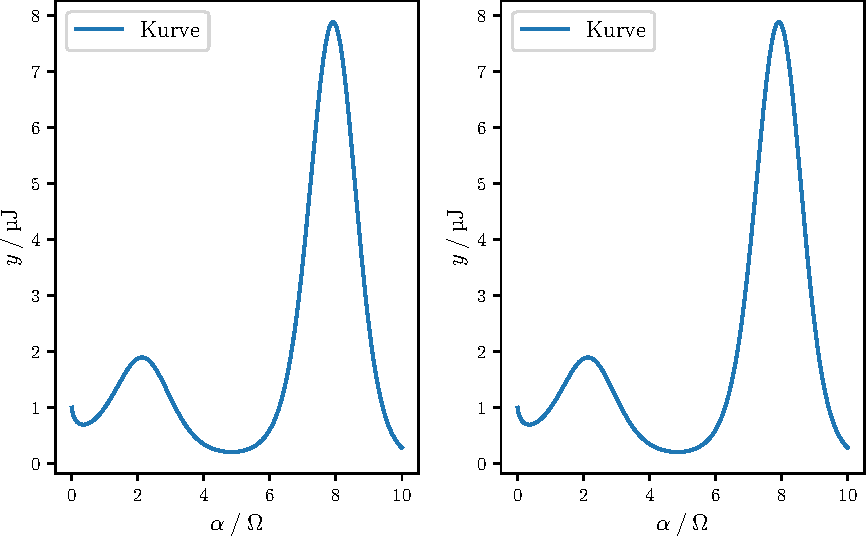
\includegraphics[width=1\textwidth]{build/plot.pdf}
  \caption{Plot der Messdaten und der Regressionskurve\protect\footnotemark}
  \label{fig:plot}
\end{figure}

%\begin{table}[!htp]
%  \centering
%  \begin{tabular}{c|c|c}
%    \toprule
%    $T [\unit{\degreeCelsius}]$ & $t_{\text{runter}} [\unit{\second}]$ & $t_{\text{hoch}} [\unit{\second}]$\\
%    \midrule
%    27.5 & 47.5 & 46\\%warum kann ich hier keine Multirow machen?????!!!!?!?!?!
%    27.5 & 45 & 43.97\\
%    29 & 43.47 & 42.97\\
%    29 & 44.13 & 42.81\\
%    30.5 & 42.19 & 41.59\\
%    30.5 & 42.4 & 41.34\\
%    32 & 41.69 & 41.12\\
%    32 & 41.91 & 40.66\\
%    39.5 & 36.03 & 35.15\\
%    39.5 & 35.41 & 35.53\\
%    47 & 32.18 & 31.03\\
%    47 & 31.66 & 30.79\\
%    50 & 30.38 & 29.97\\
%    50 & 29.91 & 29.34\\
%    52 & 28.63 & 28.22\\
%    52 & 28.91 & 28.22\\
%    56 & 27.03 & 26.53\\
%    56 & 26.88 & 26.85\\
%    \bottomrule
%  \end{tabular}
%  \label{tabellegkt}
%  \caption{Fallzeiten der großen Kugel bei steigender Temperatur}
%\end{table}
\newpage

\subsection{Berechnung der Reynoldszahl}
Zur Berechnung der Reynoldszahl wird $v = \frac{x}{t}$ \: und \: $d = 2r$ in Gleichung \eqref{eqn:5} eingesetzt.
Die Reynoldszahl der großen Kugel bei Raumtemperatur und bei $\SI{56}{\degreeCelsius}$ beträgt
\begin{align*}
  Re_{18} &= (28.27 \pm 0.21)\\
  Re_{56} &= (112.1 \pm 0.9)
\end{align*} und liegt damit unter dem kritischen Wert $R_{Krit} \approx 2300$\;\;\cite{reynold_kritisch}. Es wird mit $56\,\unit{°C}$ die höchste Temperatur benutzt, da 
die Reynoldszahl mit steigender Temperatur zunimmt und die Reynoldszahl bei der Messreihe bei $56\,\unit{°C} = T_{max}$ ihren maximalen Wert annimmt.
Die Strömung ist also laminar.\\

\newpage
%Siehe \autoref{fig:plot}!